%%%%%%%%%%%%%%%%%%%%%%%%%%%%%%%%%%%%%%%%%
% Arsclassica Article
% LaTeX Template
% Version 1.1 (1/8/17)
%
% This template has been downloaded from:
% http://www.LaTeXTemplates.com
%
% Original author:
% Lorenzo Pantieri (http://www.lorenzopantieri.net) with extensive modifications by:
% Vel (vel@latextemplates.com)
%
% License:
% CC BY-NC-SA 3.0 (http://creativecommons.org/licenses/by-nc-sa/3.0/)
%
%%%%%%%%%%%%%%%%%%%%%%%%%%%%%%%%%%%%%%%%%

%----------------------------------------------------------------------------------------
%	PACKAGES AND OTHER DOCUMENT CONFIGURATIONS
%----------------------------------------------------------------------------------------

\documentclass[
10pt, % Main document font size
a4paper, % Paper type, use 'letterpaper' for US Letter paper
oneside, % One page layout (no page indentation)
%twoside, % Two page layout (page indentation for binding and different headers)
headinclude,footinclude, % Extra spacing for the header and footer
BCOR5mm, % Binding correction
]{scrartcl}
\usepackage{enumitem}% http://ctan.org/pkg/enumitem

\newcommand\ytl[2]{
	\parbox[b]{8em}{\hfill{\color{cyan}\bfseries\sffamily #1}~$\cdots\cdots$~}\makebox[0pt][c]{$\bullet$}\vrule\quad \parbox[c]{7cm}{\vspace{7pt}\color{red!40!black!80}\raggedright\sffamily #2.\\[7pt]}\\[-3pt]}
\usepackage{tabularx}


\usepackage[]{biblatex}
\addbibresource{sample.bib}

\usepackage[pdftex,
pdfauthor={Andrea Bellani},
pdftitle={UppaalTD: a Formal Tower Defense Game (report)},
pdfsubject={Formal methods for concurrent and real-time systems},
pdfkeywords={Formal methods, concurrent systems, real-time systems, Uppaal, Politecnico di Milano},
pdfproducer={Latex with hyperref},
pdfcreator={pdflatex}]{hyperref}

%%%%%%%%%%%%%%%%%%%%%%%%%%%%%%%%%%%%%%%%%
% Arsclassica Article
% Structure Specification File
%
% This file has been downloaded from:
% http://www.LaTeXTemplates.com
%
% Original author:
% Lorenzo Pantieri (http://www.lorenzopantieri.net) with extensive modifications by:
% Vel (vel@latextemplates.com)
%
% License:
% CC BY-NC-SA 3.0 (http://creativecommons.org/licenses/by-nc-sa/3.0/)
%
%%%%%%%%%%%%%%%%%%%%%%%%%%%%%%%%%%%%%%%%%

%----------------------------------------------------------------------------------------
%	REQUIRED PACKAGES
%----------------------------------------------------------------------------------------

\usepackage[
nochapters, % Turn off chapters since this is an article        
beramono, % Use the Bera Mono font for monospaced text (\texttt)
eulermath,% Use the Euler font for mathematics
pdfspacing, % Makes use of pdftex’ letter spacing capabilities via the microtype package
dottedtoc % Dotted lines leading to the page numbers in the table of contents
]{classicthesis} % The layout is based on the Classic Thesis style

\usepackage{arsclassica} % Modifies the Classic Thesis package

\usepackage[T1]{fontenc} % Use 8-bit encoding that has 256 glyphs

\usepackage[utf8]{inputenc} % Required for including letters with accents

\usepackage{graphicx} % Required for including images
\graphicspath{{Figures/}} % Set the default folder for images

\usepackage{enumitem} % Required for manipulating the whitespace between and within lists

\usepackage{lipsum} % Used for inserting dummy 'Lorem ipsum' text into the template

\usepackage{subfig} % Required for creating figures with multiple parts (subfigures)

\usepackage{amsmath,amssymb,amsthm} % For including math equations, theorems, symbols, etc

\usepackage{varioref} % More descriptive referencing
\usepackage[left=2cm,right=2cm,top=2cm,bottom=1.5cm]{geometry}

%----------------------------------------------------------------------------------------
%	THEOREM STYLES
%---------------------------------------------------------------------------------------

\theoremstyle{definition} % Define theorem styles here based on the definition style (used for definitions and examples)
\newtheorem{definition}{Definition}

\theoremstyle{plain} % Define theorem styles here based on the plain style (used for theorems, lemmas, propositions)
\newtheorem{theorem}{Theorem}

\theoremstyle{remark} % Define theorem styles here based on the remark style (used for remarks and notes)

%----------------------------------------------------------------------------------------
%	HYPERLINKS
%---------------------------------------------------------------------------------------
 % Include the structure.tex file which specified the document structure and layout


\hyphenation{Fortran hy-phen-ation} % Specify custom hyphenation points in words with dashes where you would like hyphenation to occur, or alternatively, don't put any dashes in a word to stop hyphenation altogether

\title{\normalfont\spacedallcaps{UppaalTD: a Formal Tower Defense Game}} % The article title

\subtitle{Formal Methods for Concurrent and Real-Time Systems Homework} % Uncomment to display a subtitle

\author{\spacedlowsmallcaps{Andrea Bellani} (\href{mailto:andrea1.bellani@mail.polimi.it}{\nolinkurl{andrea1.bellani@mail.polimi.it}})}

\date{\today} % An optional date to appear under the author(s)



\begin{document}
	
	\renewcommand{\sectionmark}[1]{\markright{\spacedlowsmallcaps{#1}}}
	\lehead{\mbox{\llap{\small\thepage\kern1em\color{halfgray} \vline}\color{halfgray}\hspace{0.5em}\rightmark\hfil}}
	
	\pagestyle{scrheadings} % Enable the headers specified in this block
	
	\maketitle % Print the title/author/date block
	
	\paragraph*{Abstract}
		Uppaal is a tool for modeling, simulating and verifying real-time system as networks of timed automatons. In this report, we present our modeling and verification of the game UppaalTD (both vanilla and stochastic versions) in Uppaal. In Addition, we also present the most interesting modeling choices we discarded or adjusted in the final version of the model.
		
	\setcounter{tocdepth}{3} % Set the depth of the table of contents to show sections and subsections only
	
	\tableofcontents % Print the table of contents
	
	\listoffigures % Print the list of figures
	
	\listoftables % Print the list of tables
	
	\newpage
	
	\section{Introduction}
		\subsection{Definitions}
			\begin{itemize}
				\item \textbf{requirements} : the official specifications of UppaalTD's parameters and rules;
				\item \textbf{alive}, \textbf{targettable} or \textbf{shootable} enemy : the enemy has an health strictly greater than zero and is present on the map;
				\item \textbf{dismissed} enemy : the enemy is dead or it shot the MT and the following delay has expired;
				\item \textbf{configuration} : wave's composition and turrets configuration chosen (generalized definition from requirements one);
				\item \textbf{ending} of a wave : a wave is considered \emph{ended} when each enemy is dismissed (i.e. it can't move or shoot anymore because it has already shoot or it was killed by turrets);
				\item \textbf{location} : a location of an Uppaal template;
				\item \textbf{state} : the entire game's state in a certain time instant (i.e. each automaton's position and each variable's or clock's value);
				\item \emph{Chebyshev distance} : given two generic $n$-dimensional points $x=(x_1 \dots x_n)$ and $y=(y_1 \dots y_n)$, their Chebyshev distance can be computed as $\max\limits_{1\leq i\leq n}\{|x_i - y_i|\}$.
			\end{itemize}					
		\subsection{Project development timeline}
			\begin{table}[h!]
				\centering
				\begin{minipage}[h!]{.65\linewidth}
					\color{gray}
					\rule{\linewidth}{1pt}
					\ytl{april 8th}{First brief analysis of the requirements}
					\ytl{april 9th}{Uppaal and homework presentation}
					\ytl{april 11th}{First definition of channels and MT's template}
					\ytl{april 26th}{First definition of enemy and turret template (still not synchronized) and shoot to MT modeled with \texttt{STMTCONTROLLER}}
					\ytl{may 1st}{Complete definition of all templates and synchronization without \texttt{STMTCONTROLLER}}
					\ytl{may 15th}{First definition of queries}
					\ytl{may 17th}{Enemy compact version}
					\ytl{may 24th}{Re-design of synchronization with clocks}
					\ytl{june 15th}{First stochastic version}
					\ytl{june 24th}{Started delivery procedures}
					\ytl{june 26th}{Started report writing}
					\ytl{july 7th}{Finished report writing}
					\bigskip
					\rule{\linewidth}{1pt}%
				\end{minipage}
				\caption{Project development timeline}
			\end{table}
		\subsection{Document structure}
			Main sections:
			\begin{enumerate}
				\item \textbf{Introduction} : sum up of our definitions for the terminologies used in the document and version history of our model;
				\item \textbf{Model description} : description of the models and focus on the most critical modeling choices;
				\item \textbf{Verification results} : detailed analysis of the queries verified;
				\item \textbf{Analysis of selected configurations} : presentation and deeper analysis of the models behaviors for some interesting configurations;
				\item \textbf{Conclusions} : resume of the conclusions obtained.
			\end{enumerate}
			Appendixes:
			\begin{enumerate}
				\item[A] \textbf{Discarded choices} : presentation of the most interesting discarded design choices and the motivations behind their rejection.
			\end{enumerate}
		\subsection{Software and machines used}
			\begin{table}[h!]
				\centering
				\begin{tabular}{lll}
					\toprule
					Usage     & Software & Versioning   \\
					\midrule
					Modeling, simulation and verification & Uppaal & 5.0.0  \\
					\addlinespace
					Report writing & TeXstudio & 4.6.3 \\
					\addlinespace
					Version  & Git & 2.40.0.windows.1  \\
					\bottomrule
				\end{tabular}
				\caption{Software used}
			\end{table}
			Each query was verified used two different machines with different performances that here we briefly describe:
			\begin{table}[h!]
				\centering
				\begin{tabularx}{\textwidth}{>{\raggedright\arraybackslash}p{2.5cm} >{\raggedright\arraybackslash}p{3.5cm} >{\raggedright\arraybackslash}p{3.5cm} >{\raggedright\arraybackslash}p{3cm} >{\raggedright\arraybackslash}p{2.5cm}}
					\toprule
					Machine name & CPU & RAM & OS & Manufacturing year\\
					\midrule
					\textbf{Machine 1} & AMD Ryzen 5 3500U (2.1 GHz)  & 8 GB (5,95 GB usable) & Windows 11 Home & 2020  \\
					\addlinespace
					\textbf{Machine 2} & 11th Gen Intel(R) Core(TM) i5-1135G7 (2.4 GHz) & 24 GB (23,7 GB usable) & Windows 11 Pro & 2021\\
					\bottomrule
				\end{tabularx}
				\caption{Machine specifications}
			\end{table}
			
			This document was written over the template Arsclassica Article (\url{https://www.latextemplates.com/template/arsclassica-article}) with few adjustments by us.
	\newpage
	\section{Model description}
		We modeled both the Vanilla and the Stochastic version of the game. In particular, we firstly modeled the Vanilla version and then proceeded to modify it to model the stochastic requirements. In this section we provide a detailed explanation of both versions and how the Stochastic one was obtained from the Vanilla. We clarify that our main purpose in this section is to clarify and support our design choices rather then explain the technical aspect underlying the Uppaal code, which can be read from the templates comments.
		\subsection{Entities modeling (for Vanilla version)}
			\subsubsection{Map}
			\subsubsection{Main Tower (MT)}
			\subsubsection{Enemy}
			\subsubsection{Turret}
		\subsection{Communication modeling description (for Vanilla version)}
			\subsubsection{How turrets shoot to enemies}
			\subsubsection{How enemies shoot to the MT}
		\subsection{Enrichment of Vanilla model with stochastic features}
	\section{Verification results}
		\subsection{Vanilla model verification}
			\subsubsection{Verification without turrets}
			\subsubsection{Verification with turrets}
		\subsection{Stochastic model verification}
	\section{Analysis of selected configurations}
		\subsection{Chosen configurations for Vanilla version}
		\subsection{Chosen configurations for Stochastic version}
		\subsection{Stochastic version behaviors analysis}
		
	\subsection{Vanilla version's model}
	\subsubsection{How game's state is modeled}
	We refer as \emph{game's state} to the global state of match. It is represented by the two \texttt{\textbf{int}}:
	\begin{itemize}
		\item \texttt{left\_enemies} : in each instant, it represents the number of enemies that have not died yet;
		\item \texttt{targetable\_enemies} : in each instant, it represents the number of enemies that are currently active on the map (already spawned and alive).
	\end{itemize}
	The match is considered \emph{ended} if (and only if) \texttt{left\_enemies} is 0. In fact, \texttt{targetable\_enemies} is designed only to facilitate the process turrets use to identify enemies to shoot.
	
	\subsubsection{How communication between automatons is modeled}
	We can identify from the game's description two kind of "possible messages" sent between automatons:
	\begin{enumerate}
		\item an enemy shoots to the MT;
		\item a turret shoots to an enemy.
	\end{enumerate}
	We decided to model only "2" with a real message sent over a channel. In particular, since the MT is modeled simply as an \texttt{\textbf{int}} variable (see the \emph{Modeling of MT} section for more details), in order to shoot to it, an enemy simply decrements the variable of an amount equal to its damage.[NON SPIEGATO IL CONCETTO DELLA MUTUA ESCLUSIONE]
	
	Since there is no way in Uppaal to send a message to a precise entity in a deterministic way, a pretty easy solution we found was:
	\begin{enumerate}
		\item a turret places into the \texttt{target\_record} variable the id of the targeted enemy with the relative damage and sends a message over the broadcast channel \texttt{SHOOT\_TO\_ENEMY};
		\item each enemy that receives the message checks that the id of the target corresponds to its id and only in this case decreases its life.
	\end{enumerate}
	[SPIEGARE PROSSIMAMENTE LA QUESTIONE DELL'URGENT]
	
	\subsubsection{Modeling of MT}
	As mentioned in the previous section, MT is simply modeled as an \texttt{\textbf{int}} variable that represents MT's life. It is initially set to value defined in the requirements. For the reasons why the MT is not modeled with a template, please see the dedicated section in \emph{Discarded Choices}.
	
	\subsubsection{Modeling of Enemy}
	Enemy's template is without a doubt the most complex one:
	
	\begin{figure}[h!]
		\centering
		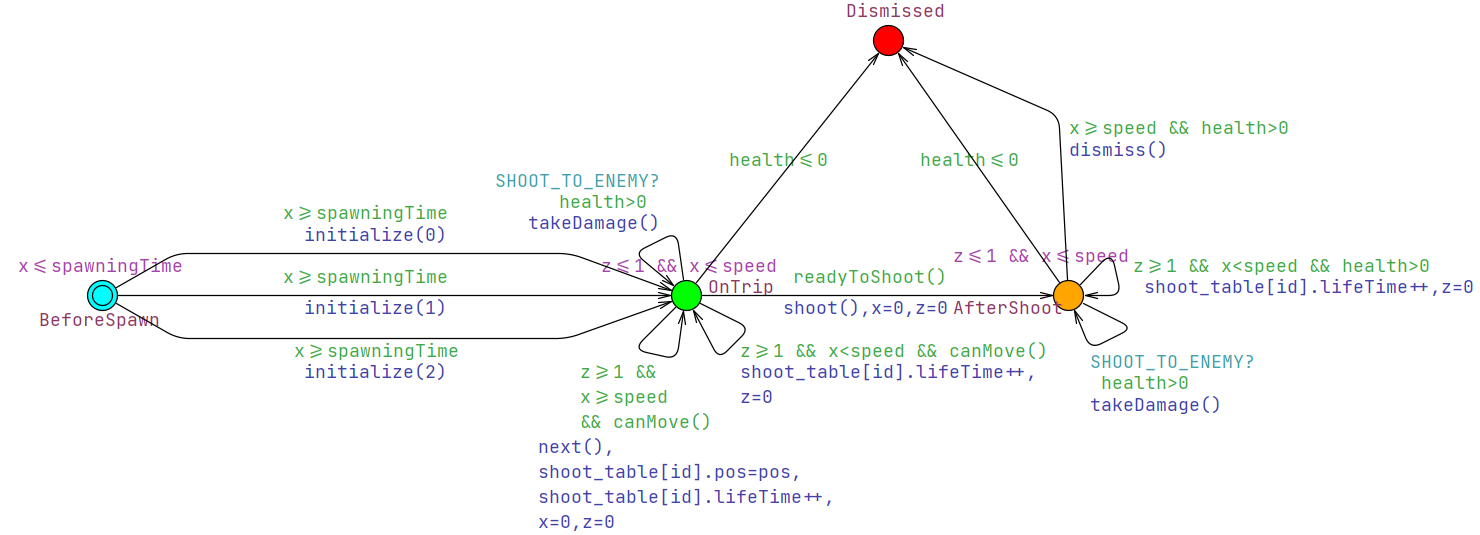
\includegraphics[width=1\textwidth]{EnemyTemplate.png}
		\caption{Enemy template}
	\end{figure}
	
	Instead of describing each state, we would rather describe how each required feature of an enemy is implemented:
	\begin{itemize}
		\item concept of \emph{spawn} : requirements state that circles should spawn at regular time intervals each other, and analogue for squares. We decided to define \texttt{spawningTime} as a parameter for an enemy, which determines the spawning timer for the enemy. So, in order to satisfy the requirements, the enemy $i$-th enemy for each kind should have this parameter set at $i*S$ (where $S$ is the spawning time defined in the requirements for that kind of enemy);
		\item how enemies move on the map : once an alive enemy is ready to move and it has not arrived at the MT spot, it calls the function \texttt{next()} which simply sets its variable \texttt{pos} to the number of the next cell from the one where it was;
		\item how non-deterministic path choice is implemented : since in a symbolic simulation, \texttt{next} can only have a deterministic execution, the non-determinism in the next cell choice in proximity of a junction is implemented simply by non-deterministically choose a number from $0$ to $2$ as soon the enemy spawns (i.e. the parameter passed to \texttt{initialize}). Then, if the enemy is in a junction, \texttt{next} chooses the next cell accordingly to this number (please see the dedicated section \emph{Discarded choices} for more details on why this design choice was preferred);
		\item how speed delay is implemented : simply, a clock $x$ is used to model the speed delay timer;
		\item how an enemy responses to a shoot : on shoot, the enemy simply decreases its life (provided that it was the target) and its life goes to zero (or beyond), \texttt{takeDamage} calls \texttt{dismiss} to set its unavailability in the shoot table and decrease the global counters. Note that the fact that \texttt{takeDamage} decrements the life counter and in case calls \texttt{dismiss} is more appropriate than always splitting the calling of \texttt{takeDamage} to the calling of \texttt{dismiss}, since it may lead having one or more time instants where a dead enemy is dead but still considered available because \texttt{takeDamage} did not update the global information;
		\item providing all information for the shoot table : the update of the shoot table from an enemy is quite trivial, apart for the field \texttt{lifeTime}, which has to be updated at each time instant (\texttt{z} clock is needed for triggering an update of it at every time instant);
		\item shoot to the MT : once an enemy reached the MT spot it simply decrements the MT life of its damage and after a delay of \texttt{speed} (where it can still be shot) is dismissed.
	\end{itemize}
	
	\subsubsection{Modeling of Turret}
	A turret has a pretty intuitive behavior:
	
	\begin{figure}[h!]
		\centering
		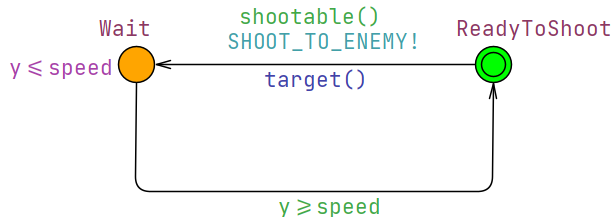
\includegraphics[width=0.5\textwidth]{TurretTemplate.png}
		\caption{Turret template}
	\end{figure}
	
	Once it is ready, it looks for targetable enemies (available enemies inside its shooting are) by scanning \texttt{SHOOT\_TABLE} with \texttt{shootable()}. If there is at least one, it uses \texttt{target()} to select and shoot the best one according to the requirements criteria:
	\begin{enumerate}
		\item \texttt{SHOOT\_TABLE} is scanned until an available enemy inside the shooting area is found and there are still available enemies in the next positions of \texttt{SHOOT\_TABLE} (\texttt{targetable\_enemies} tracks the number of currently available enemies);
		\item the found enemy is considered as the best target;
		\item the scan of the remaining elements of \texttt{SHOOT\_TABLE} is performed until the number of available enemies found is equal to \texttt{targetable\_enemies};
		\item at the end of the scan, if an enemy to target is found, the procedure \texttt{shoot} is called, which simply sets into \texttt{target\_record} the id of the targeted enemy and the relative damage (and also resets the clock \texttt{y} for the delay count). 
	\end{enumerate}
	This, perhaps not intuitive way of scanning enemies guarantees and asymptotic complexity $\Theta(MAX_ENEMIES)$, which fits our application.
	
	If the shoot succeeded, the turret stays in \texttt{Wait} until the delay expires and it can target and shoot again. Note that if all enemies are died, turrets will be in deadlock once they come back in \texttt{ReadyToShoot}.
	
	\subsection{Stochastic version's model}
	\subsubsection{Modifications from Vanilla model}
	Stochastic model is not drastically different from the Vanilla one:
	
	\begin{figure}[h!]
		\centering
		\begin{minipage}{.6\textwidth}
			\centering
			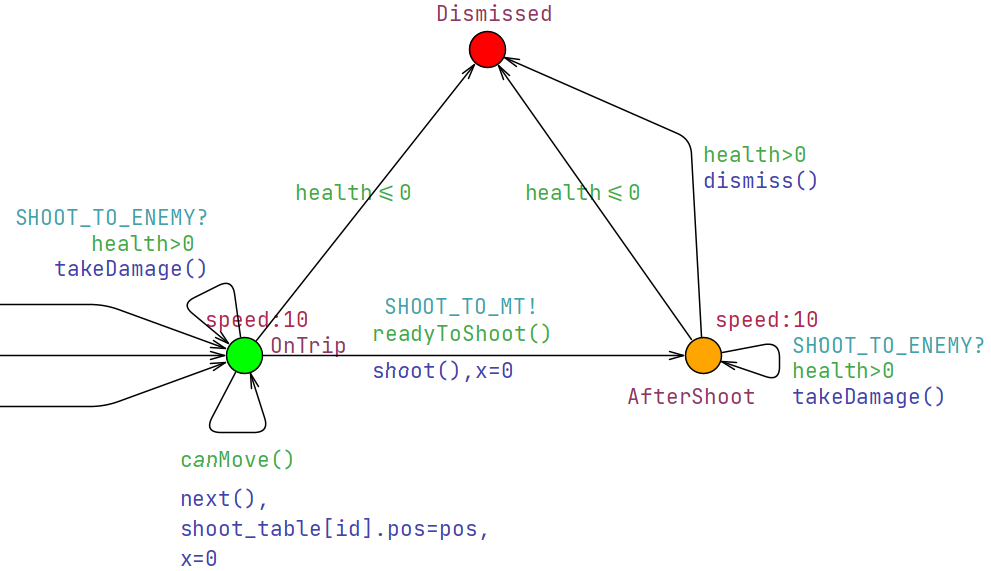
\includegraphics[width=.9\linewidth]{stochasticEnemy.png}
			\caption{Enemy stochastic template}
		\end{minipage}%
		\begin{minipage}{.4\textwidth}
			\centering
			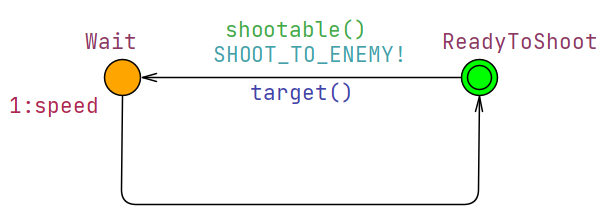
\includegraphics[width=.9\linewidth]{stochasticTurret.png}
			\caption{Turret stochastic template}
		\end{minipage}
	\end{figure}
	
	For what strictly concerns the templates:
	\begin{itemize}
		\item enemy template:
			\begin{itemize}
				\item speed delay so no more modeled as a delay but as a exponential rate that determines the probability of coming out from the state. Since while enemy is approaching the MT the only available transition (provided that the enemy is alive) is the one that calls \texttt{next}, the probability of moving to the next cell is determined by the exponential rate \texttt{speed:10}. This is analogue also in \texttt{AfterShoot};
				\item even if MT is still modeled as a variable and not as a template, an enemy that wants to shoot sends a message over the channel \texttt{SHOOT\_TO\_MT}, which simply is a \texttt{urgent broadcast} channel useful to force enemies to "not wait" before shoot when they can, otherwise also the probability of shooting to the MT at an instant would have been modeled, but requirements never ask for it, so it is better to model any outgoing transition that may change the game dynamics as \texttt{urgent} if no probabilistic delay should affect it (transition to \texttt{Dimissed} if \texttt{health$\leq$0} does not really affects game dynamics since the enemy has already died);
				\item instead of keep counting time instants to increment their \texttt{lifeTime}, enemies have their lifeTime information already determined by the instant when they spawned of the map. This simplification could also have been used in the Vanilla version but there are queries that specifically argue on how many time instants have already passed by the time an enemy arrives at the MT spot;
			\end{itemize}
		\item turret template :
			\begin{itemize}
				\item turrets firing speed is no more modeled as a delay but as an exponential rate of \texttt{1:speed} (same reasoning of the enemy's speed delay modeling);
				\item since the concept of lifetime was replaced with the entering (time instant when an enemy spawns), also turrets have to decide which enemy to shoot by using the concept of entering. Saying that younger enemies should be prioritized is equal to saying that enemies spawned later are prioritized, therefore, without loss of generality, we can use the entering information instead of lifetime.
			\end{itemize}
	\end{itemize}
	
	\section{Game configuration}
	\subsection{Vanilla version}
	\subsubsection{Configuration 1 : The unlucky side}
	\subsubsection{Configuration 2 : Sniper's inefficiency}
	\subsubsection{Configuration 3 : }
	\subsection{Stochastic version}
	\subsubsection{Configuration 1 :}
	\subsubsection{Configuration 2 :}
	\subsubsection{Configuration 3 :}
	
	\section{Verification results}
	\subsection{Queries for Vanilla version}
	\subsubsection{Queries without turrets}
	Since these query must be verified without turrets, we can assume that no enemy will die in any time instant.
	
	We interpreted the queries given as (in romans numbers, the corresponded requirements queries):
		\begin{enumerate}[label=\Roman*.]
			\item~[Q11] game is in deadlock state if and only if the match is ended;
			\item~[Q12] all enemies can reach the MT;
			\item[III, IV.]~[Q13] enemies reach the MT in no more than \texttt{MAX\_PATH\_LENGTH}$\times s$ time units (where $s$ is speed's enemy);
			\item[V.]~[Q14] an enemy must always be in a valid cell.
		\end{enumerate}
	
	Let's now analyze how we translated these natural-languages statements in Uppaal queries:
	\begin{itemize}
		\item~[Q11] game is in deadlock state if and only if the match is ended:
		
			\texttt{A[]((deadlock imply matchEnded()) and (matchEnded() imply deadlock))}
			
			
		\item~[Q12] all enemies can reach the MT:
		\item~[Q13] enemies reach the MT in no more than \texttt{MAX\_PATH\_LENGTH}$\times s$ time units (where $s$ is speed's enemy):
		\item~[Q14] an enemy must always be in a valid cell:
	\end{itemize}
	
		
	
	\subsubsection{Queries with turrets}
	\subsection{Queries for Stochastic version}
	\subsection{Consideration on efficiency}
	\subsubsection{Starting spawning instant}
	\subsubsection{Why urgent channels}
	\subsubsection{Templates parameters}
	
	
	\section{Conclusions}
	%----------------------------------------------------------------------------------------
	%	BIBLIOGRAPHY
	%----------------------------------------------------------------------------------------

	
	
	%----------------------------------------------------------------------------------------
	\newpage
	\appendix
	\section{Discarded choices}
		We wanted to write this additional section mainly to better clarify the reasons behind our final design choices. Nonetheless, we would like to clarify that our design choices are what we believed to be more efficient and adequate for our interpretation of the game, so some of the discarded can possibly be the best ones in other contexts or with different requirements and also for this reason we wanted to state them in the report.
		\subsection{MT template}
			Originally, a template for MT was designed. It was, for its simplicity, the very first one to be designed. We removed it in an attempt of optimizing the model, since we understood (after reasoning more on other more crucial design choices) that a so simple and "passive" entity like the MT does not really need to be implemented with a dedicated template (\texttt{decDamage} decreases MT's life by the value set in a global variable from the firing enemy):
			
			\begin{figure}[h!]
				\centering
				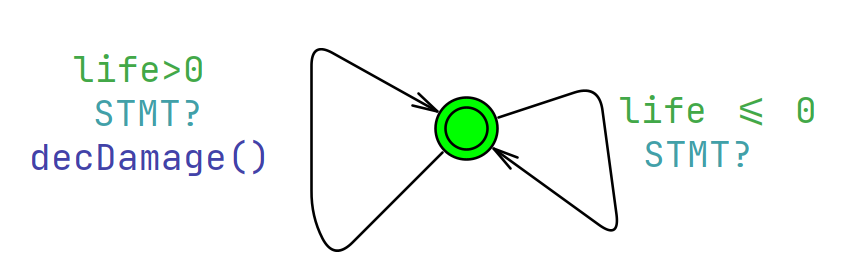
\includegraphics[width=0.5\textwidth]{MT_Template.png}
				\caption{Original MT's template}
			\end{figure}
			
			Decoupling enemy and turret in two templates is necessary to model in a proper and clear way the interleaving between these entities but MT neither needs to trigger other components nor has any non-deterministic behavior. The only one centralized aspect that a dedicated template could have implemented was controlling that MT's life is not $0$ before decreasing it, but this can be easily moved in enemy's template (before an enemy shoots, it checks that MT's life is not $0$) without loss of readability.
		\subsection{Hard-coded enemies paths}
			The very first enemy version used the concept of \texttt{next()} but there was no idea on how to model the non-deterministic moves (unless using \texttt{random()}, which is not available in symbolic simulations). The only idea was to hard-code vectors of cells representing each straight red path on the map and enemies template would have chosen between them non-deterministically with transitions (once an enemy arrives in the last cell of a path, then it will start to follow non-deterministically one of the "next paths"):
			
			\begin{figure}[h!]
				\centering
				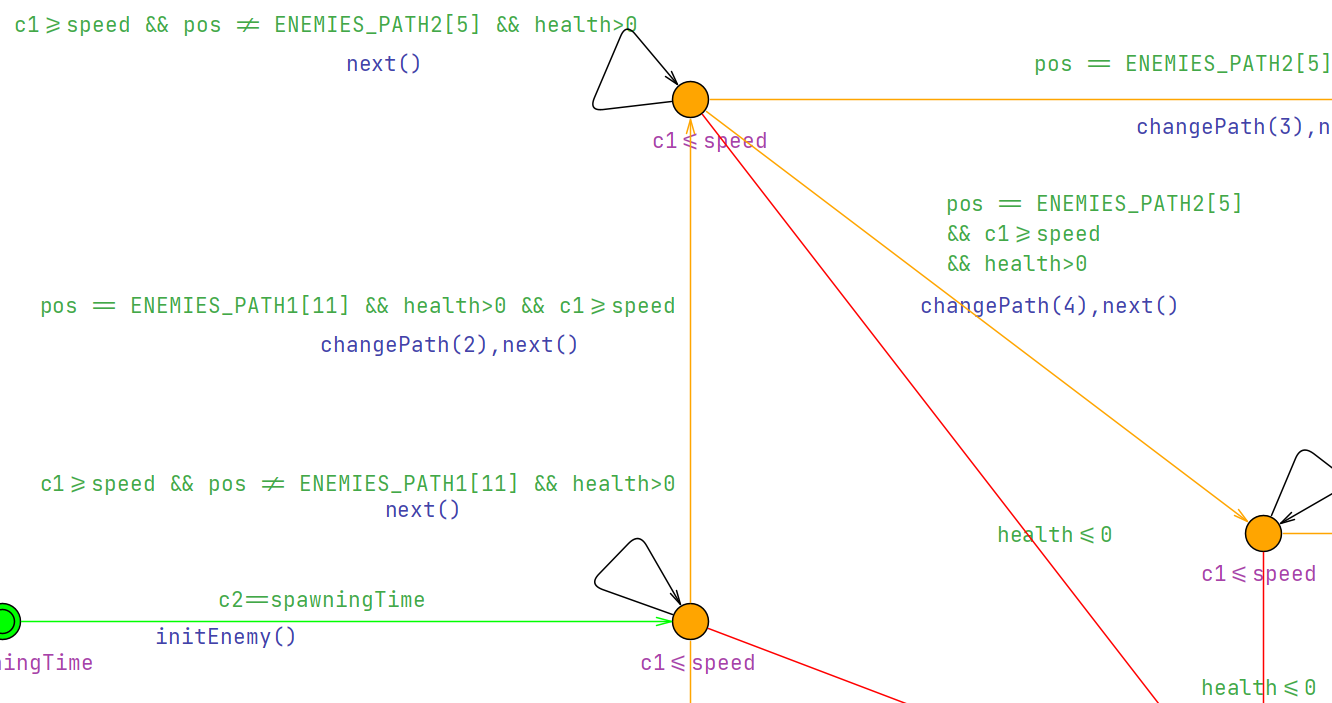
\includegraphics[width=0.65\textwidth]{ENEMIES_PATHS.png}
				\caption{Original non-deterministic path choices example}
			\end{figure}
			We realized that since during the game there is no event that may change the probability that an enemy takes a certain choice in a junction rather than another one, without loss of generality, these non-deterministic choices can be determined all at once by the time the enemy spawns (by calling \texttt{initialize()} with different parameters):
			\begin{figure}[h!]
				\centering
				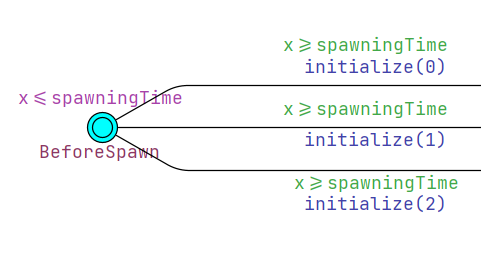
\includegraphics[width=0.65\textwidth]{COMPACT_ENEMIES_PATHS.png}
				\caption{Close-up of the non-deterministic paths choice at spawning time}
			\end{figure}
			This simple intuition really improved the readability of the enemy template (in the project development timeline we called this new version \emph{compact enemy}).
		\subsection{Quadratic enemies scanning strategy}
			The very first turret version used to look for enemies to shoot in this way: for each $k$ from $1$ to the \texttt{range}, scan \texttt{SHOOT\_TABLE} to find all the available enemies at exactly $k$ cells of distance; then, choose the best iso-distant available enemy based on the requirements criteria. The worst-case asymptotic complexity of this procedure was $\Theta(k\times MAX\_ENEMIES)$ which was significantly worse than the one of the final version which is $\Theta(MAX\_ENEMIES)$ especially in the average case where there is no enemy inside the shooting range.
		\subsection{Locks}
			At the beginning, the first way of synchronizing entities was thought in a classical lock-unlock manner:
			\begin{figure}[h!]
				\centering
				\begin{minipage}{.5\textwidth}
					\centering
					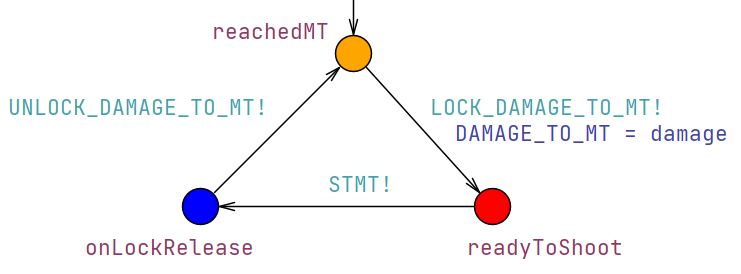
\includegraphics[width=.9\linewidth]{enemyLock.png}
					\caption{Close-up of the enemy locking \texttt{STMT} channel}
				\end{minipage}
				\begin{minipage}{.4\textwidth}
					\centering
					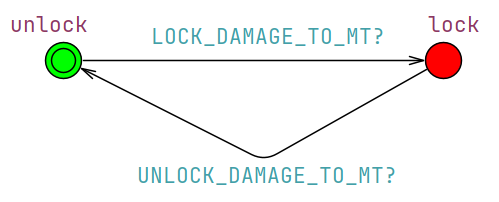
\includegraphics[width=.9\linewidth]{controller.png}
					\caption{\texttt{STMTCONTROLLER} template}
				\end{minipage}
			\end{figure}
			Once an enemy reaches the MT (for the MT template please see the proper section of the appendix):
			\begin{enumerate}
				\item the enemy sends a message to \texttt{STMTCONTROLLER} and waits for its reply (more precisely, Uppaal chooses non-deterministically which one of the ready enemies can send the message to the controller);
				\item once the controller replies the enemy places in the shared variable the damage for the MT;
				\item the enemy shoots to the MT (i.e. sends a message over \texttt{STMT});
				\item the enemy sends a message to \texttt{STMTCONTROLLER} to release the "lock".
			\end{enumerate}
			We understand that this solution is:
			\begin{itemize}
				\item deadlock-free: soon or later an acquired lock will be released and soon or later a lock request will be accepted;
				\item not starvation-free: since it is not guaranteed that any enemy that requests a lock will eventually obtain it.
			\end{itemize}
			We removed this concept since we understood that a single transition that both changes the global variable and performs the shoot would have produced the same behavior, since, provided that this transition is not synchronized with other enemies, only one of them can perform it in a time instant, therefore there is no possibility that an enemy places the damage for the MT into the shared variable and before sending the shooting message another enemy changes the variable and (or not) shoots to the MT (which would clearly create an undesired behavior).
	\nocite{1,2,3,4,5,6,7}
	\printbibliography
\end{document}